\section{Subespacioes vectoriales}
\begin{definition}{Subespacio}{subespacio} 
    Sea $V$ un $K$-espacio vectorial y $W$ un subconjunto de $V$. Decimos que $W$ es un subespacio de $V$ si:
    \begin{enumerate}[label=\alph*)]
        \item $\theta_V \in W$. \label{subespacio-p1}
        \item Si $u,v\in W$, entonces $u+v\in W$. \label{subespacio-p2}
        \item Si $\lambda \in K$ y $v\in W$, entonces $\lambda v \in W$. \label{subespacio-p3}
    \end{enumerate}
\end{definition}
\begin{notation}{}{}
    $W \leq V$ denotará que $W$ es un subespacio de $V$.
\end{notation}

\begin{example}{}{}
    \begin{enumerate}
        \item $\{(x,y,0) \mid \, x,y \in \mathbb{R}\} \leq \mathbb{R}^3 $ 
        \item $\{f: \bbR \rightarrow \bbR \mid f \text{ es continua}\} \leq \{f \mid f: \bbR \rightarrow \bbR\}$
    \end{enumerate}    
\end{example}

\begin{figure}[h]
    \centering
    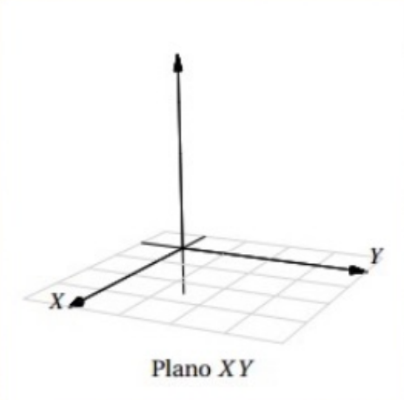
\includegraphics[scale=0.35]{src/Unidad1/img/ev1-2-1.png}
    \caption{Ejemplo de subespacio.}
    \label{fig:espacios-vectoriales2}
\end{figure}

\begin{proposition}{}{}
    Sea $V$ un $K$-espacio vectorial y $W$ un subconjunto de $V$. $W$ es un subespacio de $V$ si y solo si $W$ con las operaciones restringidas de $V$ es un $K$-espacio vectorial.
\end{proposition}
\begin{proof}
    Sea $V$ un $K$-espacio vectorial y $W$ un subconjunto de $V$. 
    $\Rightarrow$\\
    Supongamos que $W$ es un subespacio de $V$. Por el punto \ref{subespacio-p2} y \ref{subespacio-p3} de la definición \nameref{def:subespacio} la suma y el producto por escalar son cerradas en $W$, entonces las operaciones restringidas de $V$ dan una suma y un producto por escalar en $W$.\\

    Como $u+v = v+u \, \, \forall u,v \in V$, en particular $u+v = v+u \, \, \forall u,v \in W$, entonces la suma en $W$ es conmutativa. Decimos en este caso que la conmutatividad de la suma se hereda de $V$. Análogamente, se hereda la asociatividad y las propiedades 5,6,7 y 8 de espacio vectorial.\\

    Por hipótesis, $\theta_V \in W$, así $\theta_V$ funciona como neutro en $W$. Además para cada $w \in W$, $-w = (-1)w \in W$ ya que el producto es cerrado en $W$, por lo tanto se cumple la propiedad 4 de espacio vectorial.\\
    
    $\therefore W$ con las operaciones restringidas de $V$ es un $K$-espacio vectorial.\\
    
    $\Leftarrow$\\
    Supongamos que $W$ es un $K$-espacio vectorial con las operaciones restringidas de $V$, entonces la suma y el producto por escalar son cerradas en $W$ y se tienen \ref{subespacio-p2} y \ref{subespacio-p3} de la definición \nameref{def:subespacio}. Además $W$ tiene un neutro, digamos $\theta_W$\\
    \begin{align*}
        \theta_V + \theta_W &= \theta_W && \text{porque } \theta_V \text{ es neutro en } V\\
        &= \theta_W + \theta_W && \text {porque } \theta_W \text{ es neutro en } W\\
    \end{align*}
    Por \ref{prop:espacio-vectorial-cancelacion-suma} de espacio vectorial, $\theta_V = \theta_W$, por lo tanto $\theta_V \in W$.\\
    $\therefore W$ es un subespacio de $V$.
\end{proof}


\begin{obs}{}{}
    Si $V$ es un $K$-espacio vectorial, $W$ subconjunto de $V$, $W \leq V$ si y solo si se cumple:
    \begin{enumerate}
        \item $W \neq \varnothing$.
        \item $\lambda u + v \in W$ para todo $u,v \in W$ y para todo $\lambda \in K$.
    \end{enumerate}
\end{obs}


\begin{example}{}{}
    1. $V= \mathcal{M}_{n \times 1} (K), \, \, A \in \mathcal{M}_{m \times n} (K)$
    \begin{align*}
        W = \{X \in V \mid AX = 0\}
    \end{align*}
    Las soluciones del sistema homogéneo dado por $A$.
\end{example}
\begin{proof}
    P.D. $W \leq V$\\

    \begin{enumerate}
        \item $\theta_V \in W$\\
        $0 \in W$ ya que $A0 = 0$, por lo que $0 \in W$.


        \item $\lambda u + v \in W$ para todo $u,v \in W$.\\
        Sean $X_1,X_2 \in W$ veamos que $ X_1 + X_2 \in W$. 
        \begin{align*}
            A(X_1 + X_2) &= AX_1 + AX_2 && \text{por dist. de matrices} \\
            &= 0 + 0 && \text{porque } X_1,X_2 \in W\\
            &= 0
        \end{align*}
        Por lo tanto $X_1 + X_2 \in W$.\\

        \item $\lambda u \in W$ para todo $u \in W$ y para todo $\lambda \in K$.\\
        Sean $X \in W, \lambda \in K$ veamos que $\lambda X \in W$.

        \begin{align*}
            A(\lambda X) &= \lambda (AX) && \text{por prop. de matrices} \\
            &= \lambda 0 && \text{porque } X \in W\\
            &= 0
        \end{align*}
        Por lo tanto $\lambda X \in W$.
        Por lo tanto $W \leq V$.
    \end{enumerate}
\end{proof}


\begin{proposition}{}{}
    La intersección de una familia no vacía de subespacioes es un subespacio.
\end{proposition}

\begin{proof}
    Sea $V$ un $K$-espacio vectorial y $\{W_i \mid i \in I\}$ una familia no vacía de subespacios de $V$. P.D. $\bigcap_{i \in I} W_i \leq V$\\

    \begin{enumerate}
        \item Como $W_i \leq V \, \, \forall i \in I$, entonces $\theta_V \in W_i \, \, \forall i \in I$, por lo tanto $\theta_V \in \bigcap_{i \in I} W_i$.
        
        \item Sean $u,v \in \bigcap_{i \in I} W_i$, veamos que $u+v \in \bigcap_{i \in I} W_i$.\\
    \end{enumerate}
\end{proof}


\begin{definition}{Combinación Lineal}{}
    Sea $V$ un $K$ espacio vectorial. Considereamos $m \in \mathbb{N}^+$ y $v_1,\dots,v_m \in V$. Una \textbf{combinación lineal} de $v_1,\dots,v_m$ es una expresión de la forma:
    $$\lambda_1 v_1 + \cdots + \lambda_m v_m \quad \lambda_1, \cdots, \lambda_m \in K$$
    De modo más general, si $S$ es un subconjunto de $V$, una \textbf{combinación lineal de vectores de $S$} es un vector de la forma:
    $$\lambda_1 v_1 + \cdots + \lambda_m v_m \quad \lambda_1, \cdots, \lambda_m \in K, v_1,\dots,v_m \in S, m \in \mathbb{N}^+$$
\end{definition}
\begin{obs}{}{}
    Aunque el conjunto $S$ sea infinito, una combinación lineal de vectores de $S$ es una suma \textbf{finita} de vectores de $S$.
\end{obs}
\begin{proposition}
    Sea $V$ un $K$-espacio vectorial, $S \neq \varnothing$ un subconjunto de $V$. El conjunto de todas las combinaciones lineales de vectores de $S$ cumple lo siguiente:
    \begin{enumerate}[label=\alph*)]
        \item Es un subespacio de $V$.
        \item Contiene a $S$.
        \item Está contenido en cualquier subespacio de $V$ que contenga a $S$.
    \end{enumerate}
\end{proposition}


